\chapter{RESULTADOS E DISCUSSÃO}
Este capítulo é a parte principal da monografia, na qual deve apresentar os dados coletados de forma fiel e objetiva e, obrigatoriamente, realizar a discussão crítica deles, confrontando suas descobertas com o problema de pesquisa, os objetivos e o Referencial Teórico. A construção deste item exige o cruzamento de duas ações: a descrição precisa e realista dos dados obtidos, estatísticas, depoimentos ou documentos encontrados na pesquisa e a interpretação científica desses fatos, comparando os seus resultados reais com o que a literatura da área dispõe, identificando aproximações, distanciamentos e os avanços que seu estudo alcançou.

Este é um exemplo de uso de notas de rodapé. O sistema foi desenvolvido utilizando a arquitetura de microsserviços\footnote{Para mais informações acesse: \url{https://aws.amazon.com/pt/microservices/}} para garantir maior escalabilidade.

\section{Monografia Revisão de Literatura / Bibliográfica}
Optando por esse tipo de pesquisa, os resultados e a discussão consistem na análise crítica dos artigos, livros e documentos selecionados. Organize este capítulo dividindo-o em subcapítulos temáticos baseados nas categorias de análise que você encontrou nos textos estudados. Não faça apenas um resumo dos textos. Apresente os dados encontrados por outros autores, aponte onde as pesquisas deles se aproximam (convergências), onde eles divergem (divergências) e qual é o posicionamento crítico sobre o tema.

\section{Monografia Pesquisa de Campo / Estudo de Caso}
Optando por esse tipo de pesquisa, analisará os dados reais coletados na escola, empresa ou comunidade. Você pode organizar a apresentação por meio de Categorias de Análise (eixos temáticos extraídos dos dados). Sempre que houver dados estatísticos ou quantificáveis, utilize tabelas, quadros ou gráficos apropriados, inserindo título na parte superior e fonte na parte inferior (Normas ABNT).

\begin{figure}[htb]
    \centering
	\caption{\label{fig:bpmn-modelagem}Representação da estrutura do Spring Data}
    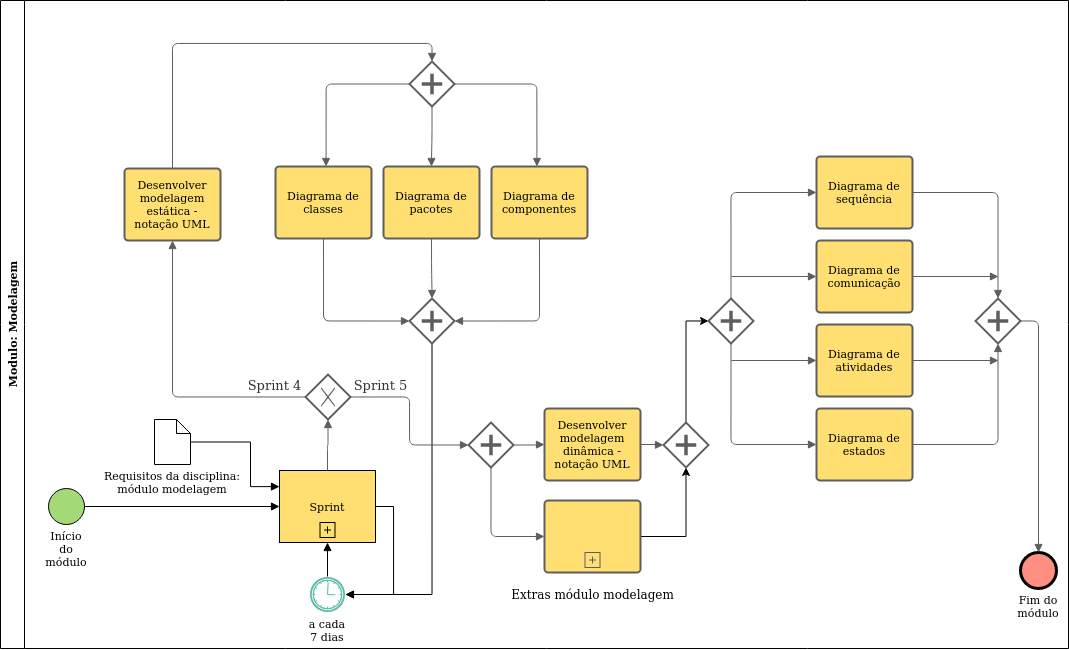
\includegraphics[width=0.85\linewidth]{img/bpmn_modelagem.png}
	\fonte{\citeonline{ribeiro2015beneficios}}
\end{figure}

\begin{table}[htb]
\centering
\caption{Exemplo de tabela de acompanhamento de atividades}
\begin{tabular}{|l|c|c|c|c|c|c|c|}
\hline
\textbf{Atividades / Meses} & \textbf{Jun} & \textbf{Jul} & \textbf{Ago} & \textbf{Set} & \textbf{Out} & \textbf{Nov} & \textbf{Dez} \\ \hline
Levantamento bibliográfico & X & & & & & & \\ \hline
Pesquisa de campo & & X & X & & & & \\ \hline
Aplicação do instrumento & & & X & X & & & \\ \hline
Análise dos dados & & & & X & X & & \\ \hline
Redação da monografia & & & & & X & X & \\ \hline
Apresentação & & & & & & & X \\ \hline
\end{tabular}
\fonte{Elaborado pelo autor (\the\year).}
\end{table}
